\documentclass[a4paper,slidestop,xcolor=pst,blue]{beamer}

\usepackage{beamerthemesplit}
\usepackage[utf8]{inputenc}
\usepackage[spanish]{babel}
\usepackage{graphicx}
\usepackage{pstricks} % PSTricks package
\usepackage{setspace}
\usepackage{multirow}
\usepackage{listings}
\usepackage{pgfpages}
\usepackage{hyperref}
\usepackage{etoolbox}
\usepackage{epstopdf}

\makeatletter
\patchcmd{\beamer@sectionintoc}{\vskip1.5em}{\vskip0.5em}{}{}
\makeatother

\setbeamercovered{dynamic}
\setcounter{tocdepth}{2}
\setbeamercolor{frametitle}{fg=black,bg=white}
\setbeamercolor{section in toc shaded}{fg=black}
\setbeamercolor{section in toc}{fg=red}
\setbeamercolor{subsection in toc shaded}{fg=black}
\setbeamercolor{subsection in toc}{fg=red}
\setbeamerfont{section in toc}{size=\small}
\setbeamerfont{subsection in toc}{size=\small}
\setbeamertemplate{section in toc shaded}[default][99]
\setbeamertemplate{subsection in toc shaded}[default][99]

\AtBeginSection[]
{\begin{frame}[c]
  \frametitle{Índice}
	\tableofcontents[currentsection,
        sectionstyle=show/shaded,
        subsectionstyle=hide]
\end{frame}}

\AtBeginSubsection[]
{\begin{frame}[c]
	\frametitle{Índice}
	\tableofcontents[
  		currentsection,
  		sectionstyle=shaded/shaded,
  		currentsubsection,
  		subsectionstyle=show/shaded/hide
		]
\end{frame}}

\setbeamercolor{frametitle}{fg=black,bg=white}

\setbeamertemplate{frametitle}{
	\begin{centering}
		\insertframetitle
		\par
	\end{centering}
}

\usetheme[secheader]{Boadilla} 

\title[Introducci�n a las Arq. Empresariales]{Introducci�n a las Arquitecturas Empresariales}

\author[P. S�nchez]{\alert{Pablo S�nchez}}

\institute[IIE]{
		   Dpto. Ingenier�a Inform�tica y Electr�nica \\
		   Universidad de Cantabria \\
		   Santander (Cantabria, Espa�a) \\
		   \texttt{p.sanchez@unican.es}
}

\date{}

\begin{document}

\begin{frame}[c]
	\titlepage
	\begin{columns}
		\column{0.50\linewidth}
			\centering
    		
\includegraphics[width=.28\textwidth,keepaspectratio=true]{images/istr.eps}
		\column{0.50\linewidth}
			\centering
			
\includegraphics[width=.25\textwidth,keepaspectratio=true]{images/uc.eps}
	\end{columns}
\end{frame}

\begin{frame}[c]
    \frametitle{\alert{Advertencia}}
    \begin{center}
        Todo el material contenido en este documento no constituye en modo alguno una obra de referencia o apuntes oficiales mediante el cual se puedan preparar las pruebas evaluables necesarias para superar la asignatura. \ \\
        \ \\
        Este documento contiene exclusivamente una serie de diapositivas cuyo objetivo es servir de complemento visual a las actividades realizadas en el aula para la transmisi�n del contenido sobre el cual versar�n las mencionadas pruebas evaluables.  \ \\
        \ \\
        Dicho de forma m�s clara, \alert{estas transparencias no son apuntes y su objetivo no es servir para que el alumno pueda preparar la asignatura.}
    \end{center}
\end{frame}

\section{Introducci�n}

\subsection{Objetivos y Bibliograf�a}

\begin{frame}[c]
    \frametitle{Objetivos del Tema}
    \begin{enumerate}[<+->]
         \item Comprender en profundidad cu�les son las responsabilidades de la capa de dominio.
         \item Conocer los principales patrones relacionados con el desarrollo de una capa de dominio.
         \item Conocer las ventajas e inconvenientes del patr�n \emph{Domain Model}.
         \item Ser capaz de aplicar el patr�n \emph{Domain Model}.
         \item Ser capaz de aplicar los principios de \emph{Domain-Driven Design}.
    \end{enumerate}
\end{frame}

\begin{frame}[c]
    \frametitle{Bibliograf�a}
    \begin{thebibliography}{1}

        \bibitem[Fowler, 2002]{Fowler2002x}
        Fowler, M. (2002).
        \newblock {\em {Patterns of Enterprise Application Architecture}}.
        \newblock Addison-Wesley.

        \bibitem[Evans, 2013]{Evans2003}
        Evans, E. J. (2003).
        \newblock {\em {Domain-Driven Design}}.
        \newblock Addison-Wesley.

        \bibitem[Esposito and Saltarello, 2014]{Esposito2014}
        Esposito, D. and Saltarello, A. (2014).
        \newblock {\em {Microsoft .NET - Architecting Applications for the
          Enterprise}}. 2� Ed..
        \newblock Microsoft Press

    \end{thebibliography}
\end{frame}

\subsection{Contexto: Capa de Dominio}

\begin{frame}[c]
    \frametitle{Capa de Dominio}
    \begin{center}
        \only<1|handout:0>{
            \rput[lt](0,0){
                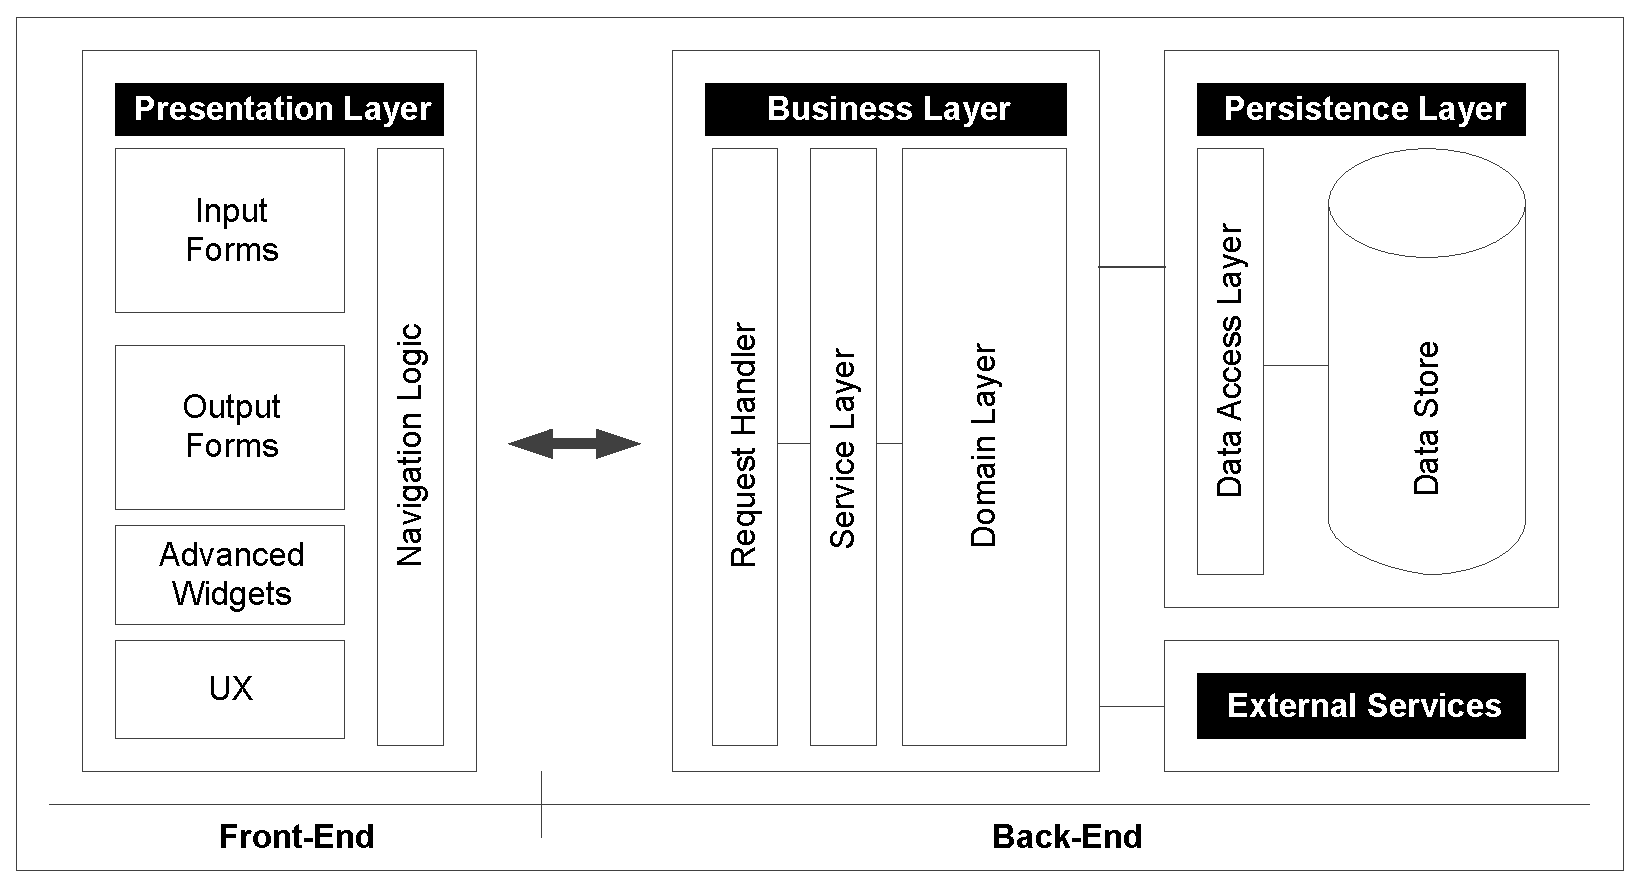
\includegraphics[width=\linewidth]{images/introduccion/enterpriseArchitectures00.eps}
            }
        }
        \only<1|handout:0>{
            \rput[lt](0,0){
                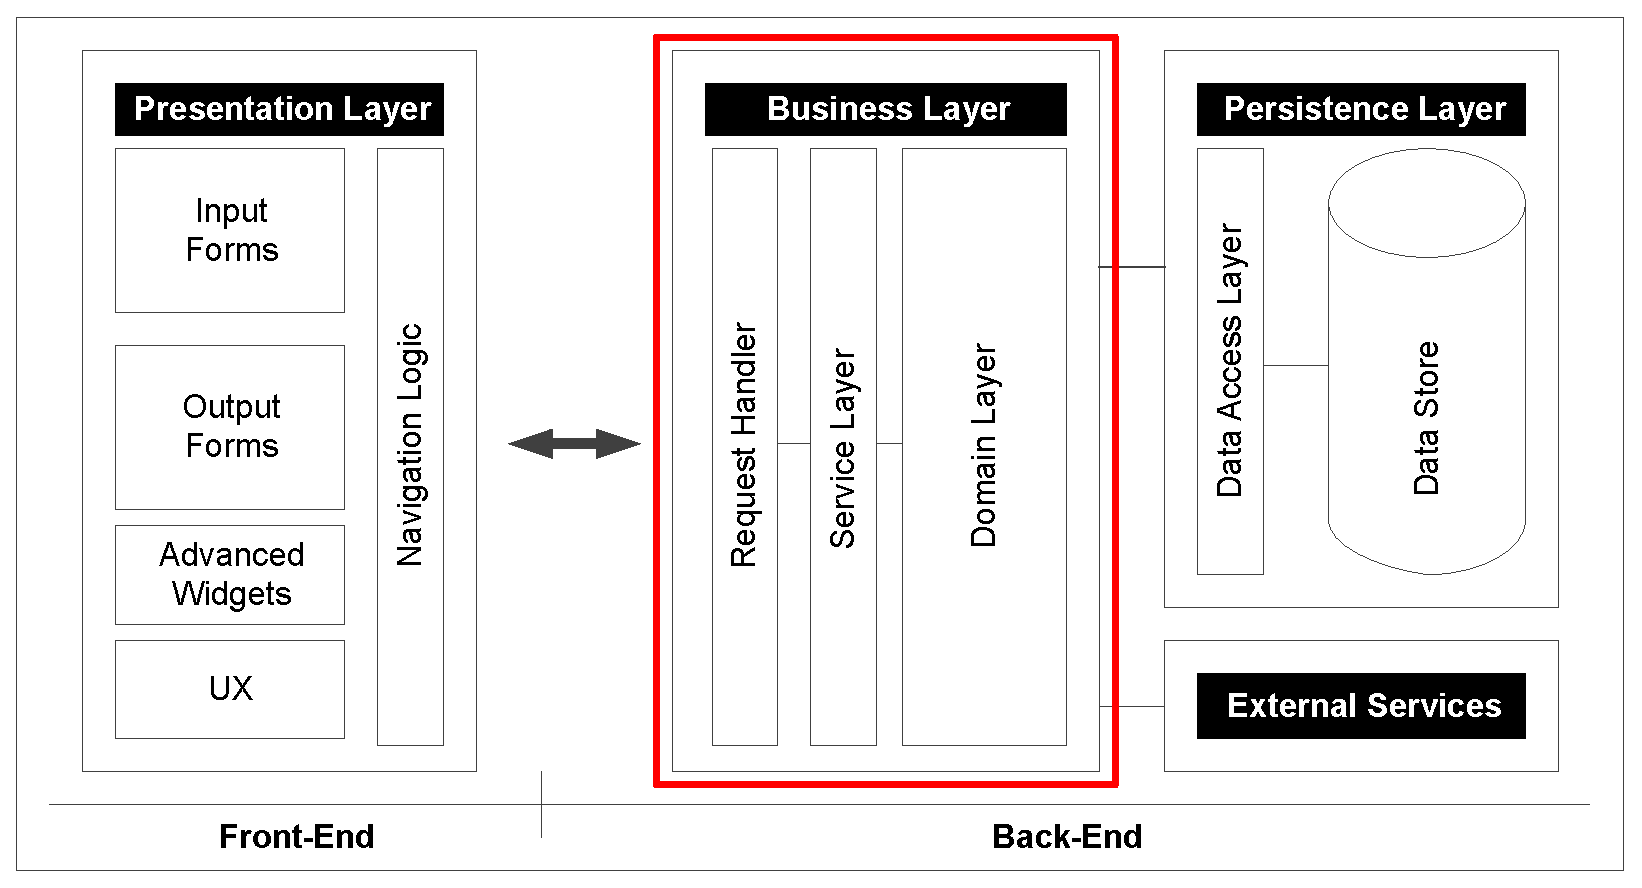
\includegraphics[width=\linewidth]{images/introduccion/enterpriseArchitectures01.eps}
            }
        }
        \only<1|handout:0>{
            \rput[lt](0,0){
                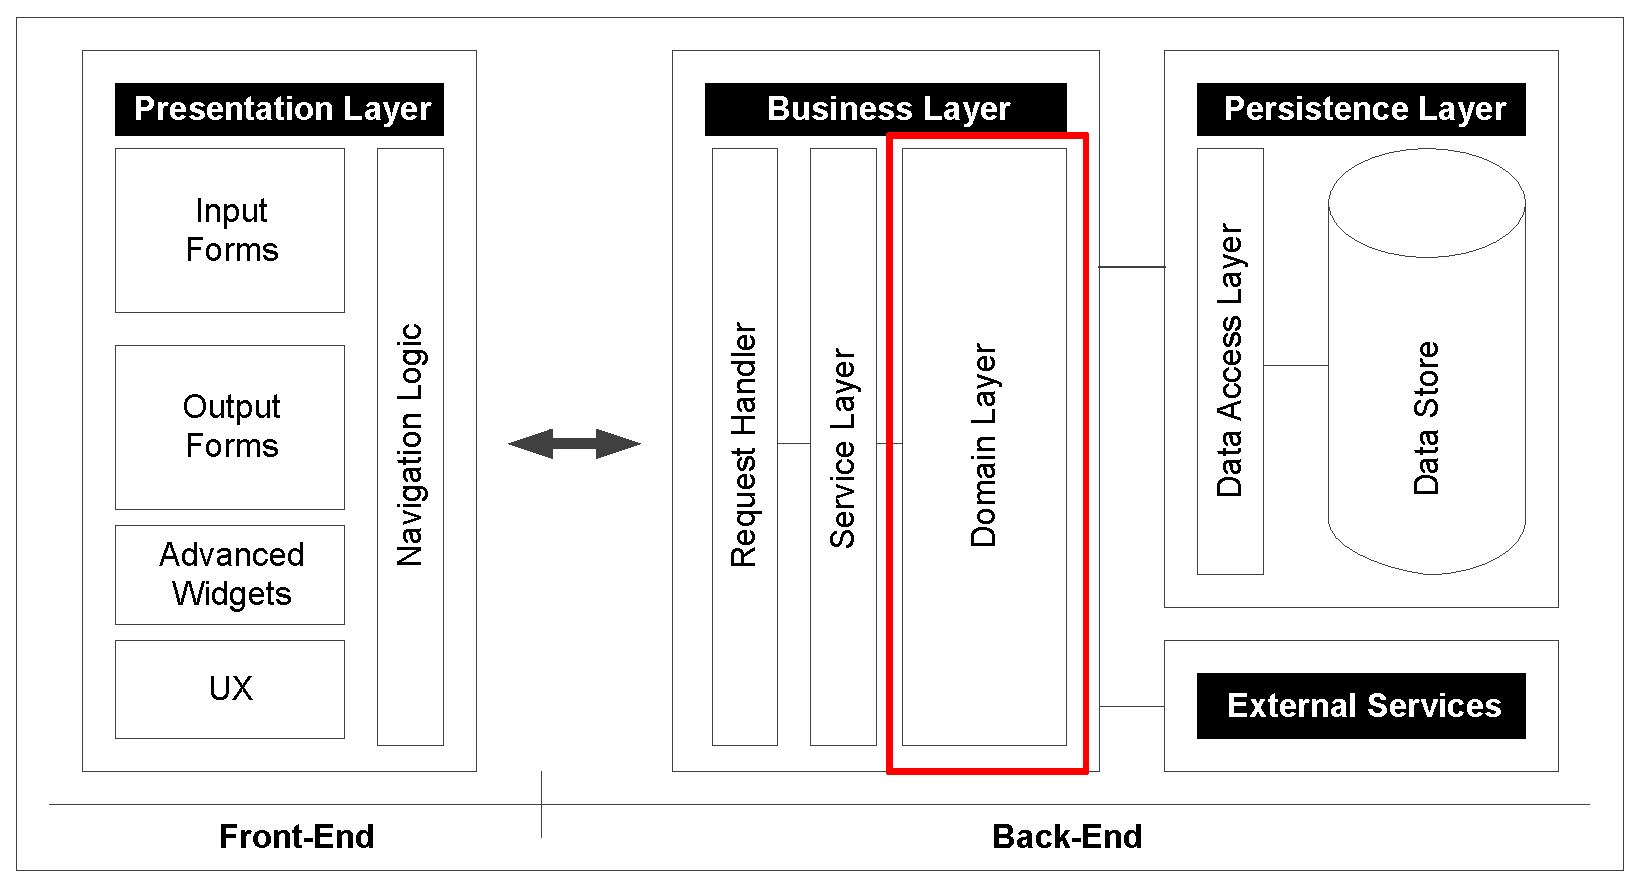
\includegraphics[width=\linewidth]{images/introduccion/enterpriseArchitectures02.eps}
            }
        }
    \end{center}
\end{frame}

\begin{frame}
    \frametitle{Responsabilidades de la Capa de Dominio}
	\begin{enumerate}[<+->]
        \item Atender las peticiones de los clientes.
        \item Asegurar que las peticiones se gestionan de acuerdo con las \alert{reglas de negocio} existentes.
        \item Validar las peticiones de los clientes.
        \item Controlar la seguridad de las operaciones.
        \item Recuperar y almacenar datos del almac�n o almacenes persistentes.
        \item Gestionar la comunicaci�n con los servicios externos.
        \item Asegurar la \alert{transacionalidad} de las operaciones.
        \item Gestionar de manera adecuada casos excepcionales.
        \item Ejecutar operaciones peri�dicas de mantenimiento.
        \item Facilitar la interconexi�n con otros sistemas.
        \item Facilitar la eficiencia del sistema.
        \item Ayudar a mejorar la experiencia de usuario.
	\end{enumerate}
\end{frame}

\section{Patrones para la Capa de Dominio}

\subsection{Table Module}

%\begin{frame}
%    \framtitle{Antipatr�n \emph{Smart UI}}
%
%    %% Put all the business logic into the user interface. Chop the application into
%    %% small functions and implement them as separate user interfaces, embedding
%    %% the business rules into them. Use a relational database as a shared repository of
%    %% the data. Use the most automated UI building and visual programming tools available.
%
%Advantages
%Productivity is high and immediate for simple applications.
%Less capable developers can work this way with little training.
%Even deficiencies in requirements analysis can be overcome by releasing a prototype to users
%and then quickly changing the product to fit their requests.
%Applications are decoupled from each other, so that delivery schedules of small modules can
%be planned relatively accurately. Expanding the system with additional, simple behavior can
%be easy.
%Relational databases work well and provide integration at the data level.
%4GL tools work well.
%When applications are handed off, maintenance programmers will be able to quickly redo
%portions they can't figure out, because the effects of the changes should be localized to each
%particular UI.
%Disadvantages
%Integration of applications is difficult except through the database.
%There is no reuse of behavior and no abstraction of the business problem. Business rules
%have to be duplicated in each operation to which they apply.
%Rapid prototyping and iteration reach a natural limit because the lack of abstraction limits
%refactoring options.
%Complexity buries you quickly, so the growth path is strictly toward additional simple
%applications. There is no graceful path to richer behavior.
%\end{frame}
%
%\begin{frame}
%    \frametitle{Table Module (deprecated)}
%    \begin{block}{Problema}
%        \begin{enumerate}{}
%        \end{enumerate}
%    \end{block}
%\end{frame}

\begin{frame}
    \frametitle{Table Module}
     TODO
\end{frame}

\subsection{Transaction Script}

\begin{frame}
    \frametitle{Transaction Script}
     TODO   
\end{frame}

\subsection{Domain Model + Service Layer}

\begin{frame}
    \frametitle{Domain Model}
     TODO
\end{frame}

\begin{frame}
    \frametitle{Service Layer}
     TODO
\end{frame}

\section{Domain-Driven Design}

\subsection{Introducci�n}

\begin{frame}[c]
    \frametitle{Domain-Driven Design}
     \begin{block}{Domain-Driven Design}
     \alert{Domain-Driven Design} es una t�cnica de desarrollo sw donde todo el dise�o de un producto sw gira en torno a un elemento central y fundamental que es el \emph{modelo de dominio}, el cual captura el dominio y la l�gica de negocio de dicho producto sw. 
     \end{block}
      %% Contar la historia de Monty Python
      %% Contar la historia del PCB
      
      %% Ventajas e Incovenientes: https://goo.gl/gPx5DE
\end{frame}

\begin{frame}[c]
    \frametitle{Domain-Driven Design}
     \begin{block}{Ubiquitous Language}
     TODO
     \end{block}
     %% Leer Cap�tulo 3 de Evans
\end{frame}

\begin{frame}[c]
    \frametitle{Domain-Driven Design}
     \begin{block}{Entities}
     TODO
     \end{block}
     %% Leer Cap�tulo 3 de Evans
\end{frame}


\section{Sumario y Conclusiones}

\end{document}
